\chapter{安装与输入源注册：为什么复制应用还不够}

\begin{goals}
理解输入法安装位置、输入源注册和系统缓存；区分开发目录副本、DMG 副本与已安装副本；能够设计幂等、自愈且不破坏用户数据的安装流程。
\end{goals}

普通 macOS 应用可以从 Applications 目录启动，输入法还要被文本输入系统发现。MyIME 采用当前用户安装，把自身复制到 \sourcefile{~/Library/Input Methods/MyIME.app}，注册输入源，再从安装位置重新启动。这样不需要管理员权限，也避免开发构建与正式输入服务并存。

\figmp{10}{从 DMG 到 IMKServer 的输入源生命周期}

\section{幂等安装}

理想安装器重复运行不会制造多个副本或多个登录项。它应先解析自身位置和目标位置，比较版本，安全替换目标，注册输入源，移除历史机制，再启动目标副本。任何删除都必须使用已经解析并验证的具体路径。

\lstinputlisting[language=Swift,firstline=1,lastline=110,caption={SelfInstaller 的路径、命令和已安装副本判断}]{../../MyIME/MyIME/App/SelfInstaller.swift}

\section{同一 Bundle ID 的多个副本}

当 \sourcefile{/Library/Input Methods} 与 \sourcefile{~/Library/Input Methods} 同时存在相同 Bundle ID，LaunchServices/TIS 可能缓存错误副本。用户看到同名菜单项，却不确定系统启动了哪个路径。升级时因此要检测和迁移旧的系统级副本。

\section{App Translocation}

从下载位置直接打开未正确处理的应用，macOS 可能通过随机只读路径运行它。输入法若把这个临时路径当作稳定安装位置，重新启动和自更新会形成循环。工程代码必须只在确认已位于目标目录后建立服务器；安装阶段完成复制后，从确定路径启动。

\lstinputlisting[language=Swift,firstline=110,lastline=250,caption={安装准备、复制替换与目标副本重启}]{../../MyIME/MyIME/App/SelfInstaller.swift}

\begin{warningbox}[安装器是高风险代码]
安装器会复制、替换甚至清理旧应用。必须验证目标是具体的 MyIME.app，禁止对宽泛目录递归删除；失败时保留原可用版本；不要因为“只在自己电脑测试”而忽略恢复路径。
\end{warningbox}

\begin{lab}[幂等性]
连续运行安装器三次，记录输入源数量、安装路径、进程路径和用户数据库校验和。通过标准是没有重复输入源、进程始终来自目标路径、用户库不变。
\end{lab}

\exercises
\begin{enumerate}
  \item 为什么 DMG 中双击应用后不应直接把该副本作为长期输入服务？
  \item 设计一次失败替换后的回滚方案。
  \item 如何证明系统当前启动的确实是新版本而非缓存旧副本？
\end{enumerate}

\begin{summarybox}
输入法安装是“复制＋注册＋选择＋启动”的事务。路径稳定、单副本、幂等和失败恢复比漂亮的安装窗口更重要。
\end{summarybox}


\chapter{InputMethodKit 的多条事件路径}

\begin{goals}
识别 \code{handle}、\code{inputText} 与文本数据模式；理解不同客户端为何表现不同；能够在不复制业务逻辑的前提下统一事件处理。
\end{goals}

真实输入法常见现象是 Notes 正常、某个 WebKit 页面失败，或者开发机正常、目标机无法输入中英文。根源未必在词库，而可能是 IMKServer 的输入模式、客户端协议实现和事件投递路径不同。

MyIME 1.0.10 对“text data only”投递做了适配：系统可能不调用常见的 \code{handle(_:client:)} 或 \code{inputText(_:client:)}，而通过包含 Unicode、硬件键码和修饰符的文本数据入口提供事件。

\lstinputlisting[language=Swift,firstline=138,lastline=255,caption={文本数据投递路径与统一按键处理}]{../../MyIME/MyIME/Controller/MyIMEInputController.swift}

\section{统一语义，不统一假设}

三条入口最终应转换成相同的语义动作，但不能假设每条入口都提供完全相同的信息。NSEvent 可能包含键盘布局后的字符与 flags；文本数据可能只含特定字段；安全输入环境可能限制内容。适配层应明确哪些字段缺失，以及缺失时选择放行还是降级处理。

\section{客户端协议差异}

原生 NSTextView、浏览器网页输入框和 Electron 编辑器都声称支持文本输入协议，但对 replacementRange、marked range、selected range 和窗口坐标的实现细节可能不同。避免依赖“恰好在 Notes 可用”的未声明行为，例如：

\begin{itemize}
  \item 不应假设 marked range 永远有效；
  \item replacementRange 未知时使用 \code{NSNotFound} 语义；
  \item 客户端切换后不复用旧对象；
  \item 坐标查询失败时隐藏候选窗而不是崩溃；
  \item 提交和清空顺序在所有路径保持一致。
\end{itemize}

\begin{lab}[事件路径日志]
为三个入口分别增加只记录方法名、键码和修饰符的 Debug 日志。在 Notes、Safari、Chrome 和 Electron 应用中输入同一序列，形成对照表。Release 构建不得记录完整文本。
\end{lab}

\exercises
\begin{enumerate}
  \item 为什么“某方法没有被调用”不能直接解释为输入法进程没有运行？
  \item 如何避免三条入口复制三份退格与选词逻辑？
  \item 客户端不给有效插入点坐标时，候选窗口应怎样降级？
\end{enumerate}

\begin{summarybox}
InputMethodKit 适配的核心是把多条不完全等价的系统入口转换成统一动作，同时保留缺失信息和客户端差异的证据。
\end{summarybox}


\chapter{组合会话、失活恢复与幽灵状态}

\begin{goals}
理解输入源切换、应用切换和控制器失活对组合状态的影响；能够避免幽灵候选、跨应用误提交和旧客户端引用；设计清晰的恢复策略。
\end{goals}

输入法状态不仅被按键改变，也被系统生命周期改变。用户可以在组合中点击别的窗口、切换输入源、锁屏、结束进程或打开设置。若控制器只在 \key{Space} 和 \key{Esc} 时清理状态，就会留下“幽灵组合”。

MyIME 对 \code{commitComposition}、失活和输入源变化分别处理，并保存弱引用以便最终清理滞留组合。

\lstinputlisting[language=Swift,firstline=256,lastline=330,caption={提交组合、控制器失活和会话清理}]{../../MyIME/MyIME/Controller/MyIMEInputController.swift}

\section{策略矩阵}

\begin{center}
\begin{tabular}{p{3cm}p{3cm}p{5cm}}
\toprule
事件 & 推荐默认 & 风险 \\
\midrule
按 Esc & 取消 & 用户预期明确 \\
按 Return & 提交当前选择/原文 & 需区分导航状态 \\
切换输入源 & 提交或取消，保持一致 & 旧 marked text 滞留 \\
客户端失活 & 结束当前组合 & 不能提交到新客户端 \\
进程异常结束 & 由系统清理 & 文档可能保留显示残影 \\
\bottomrule
\end{tabular}
\end{center}

没有一种策略适合所有产品，但策略必须一致、可测试并写入用户说明。尤其不能让“失活时提交首选”和“输入源切换时取消”在用户无感知的情况下互相矛盾。

\section{弱引用与所有权}

输入法不拥有客户端生命周期。长时间强引用旧客户端可能导致泄漏或错误调用。弱引用允许控制器在必要时清理，同时接受客户端已经消失。所有回调都应在使用前重新确认客户端能力。

\begin{lab}[幽灵状态测试]
输入 \code{nihao} 但不上屏，依次执行：切换窗口、切换输入源、关闭文档、强制结束进程。每个场景重新激活 Notes，确认候选窗和 raw 不会复活，也不会把“你好”写入错误文档。
\end{lab}

\exercises
\begin{enumerate}
  \item 失活时提交原始拼音和取消组合各有什么优缺点？
  \item 为什么全局静态变量保存“当前客户端”风险很高？
  \item 设计一个可用状态转移表自动生成的生命周期测试。
\end{enumerate}

\begin{summarybox}
输入法组合是一段与客户端绑定的会话。生命周期事件必须显式结束会话，旧状态和旧客户端都不能跨越新的焦点边界。
\end{summarybox}


\chapter{日志、诊断与证据链}

\begin{goals}
建立分层日志类别；掌握从输入源状态到候选生成的证据链；在保护隐私的前提下定位“无法输入”和“候选错误”。
\end{goals}

输入法错误经常发生在用户看不到的后台进程。弹窗会抢焦点，\code{print} 输出又未必容易找到，因此应使用统一日志系统，并按 bootstrap、installer、controller、engine、store 分类。

\section{用 Logger 建立可过滤日志}

统一日志的首要价值不是“多打印一些文字”，而是把来源、严重级别和隐私属性变成结构化字段。所有模块使用相同 subsystem，再用 category 区分职责：

\begin{lstlisting}[language=Swift,caption={结构化、可过滤且默认脱敏的统一日志}]
import OSLog

private let log = Logger(
    subsystem: "fudan.miniS.MyIME",
    category: "controller"
)

log.debug("keyDown keyCode=\(event.keyCode) session=\(sessionID, privacy: .public)")
log.info("candidates count=\(candidates.count) latencyMs=\(elapsedMs)")
log.error("store unavailable code=\(errorCode, privacy: .public)")
\end{lstlisting}

只有不含正文、不会识别个人的字段才标记 \code{.public}。原始拼音、候选文本和提交句子保持 private 或根本不写入；Debug 构建也不应形成“先泄露、发布前再删除”的习惯。

\section{Console.app 过滤 SOP}

打开“应用程序→实用工具→控制台”，选中当前 Mac 并点击“开始流式传输”。在搜索框输入 \code{fudan.miniS.MyIME}，把匹配项类型改成 \textbf{Subsystem}；需要缩小范围时，再加 \textbf{Category} 为 \code{controller}、\code{bootstrap} 或 \code{installer}。打开“包括信息信息”和“包括调试信息”，清空旧视图后复现一次，再立即暂停。图中的蓝色 \textsc{SUBSYSTEM} 令牌说明过滤条件已被 Console 识别，而不是普通全文搜索。

\begin{figure}[htbp]
  \centering
  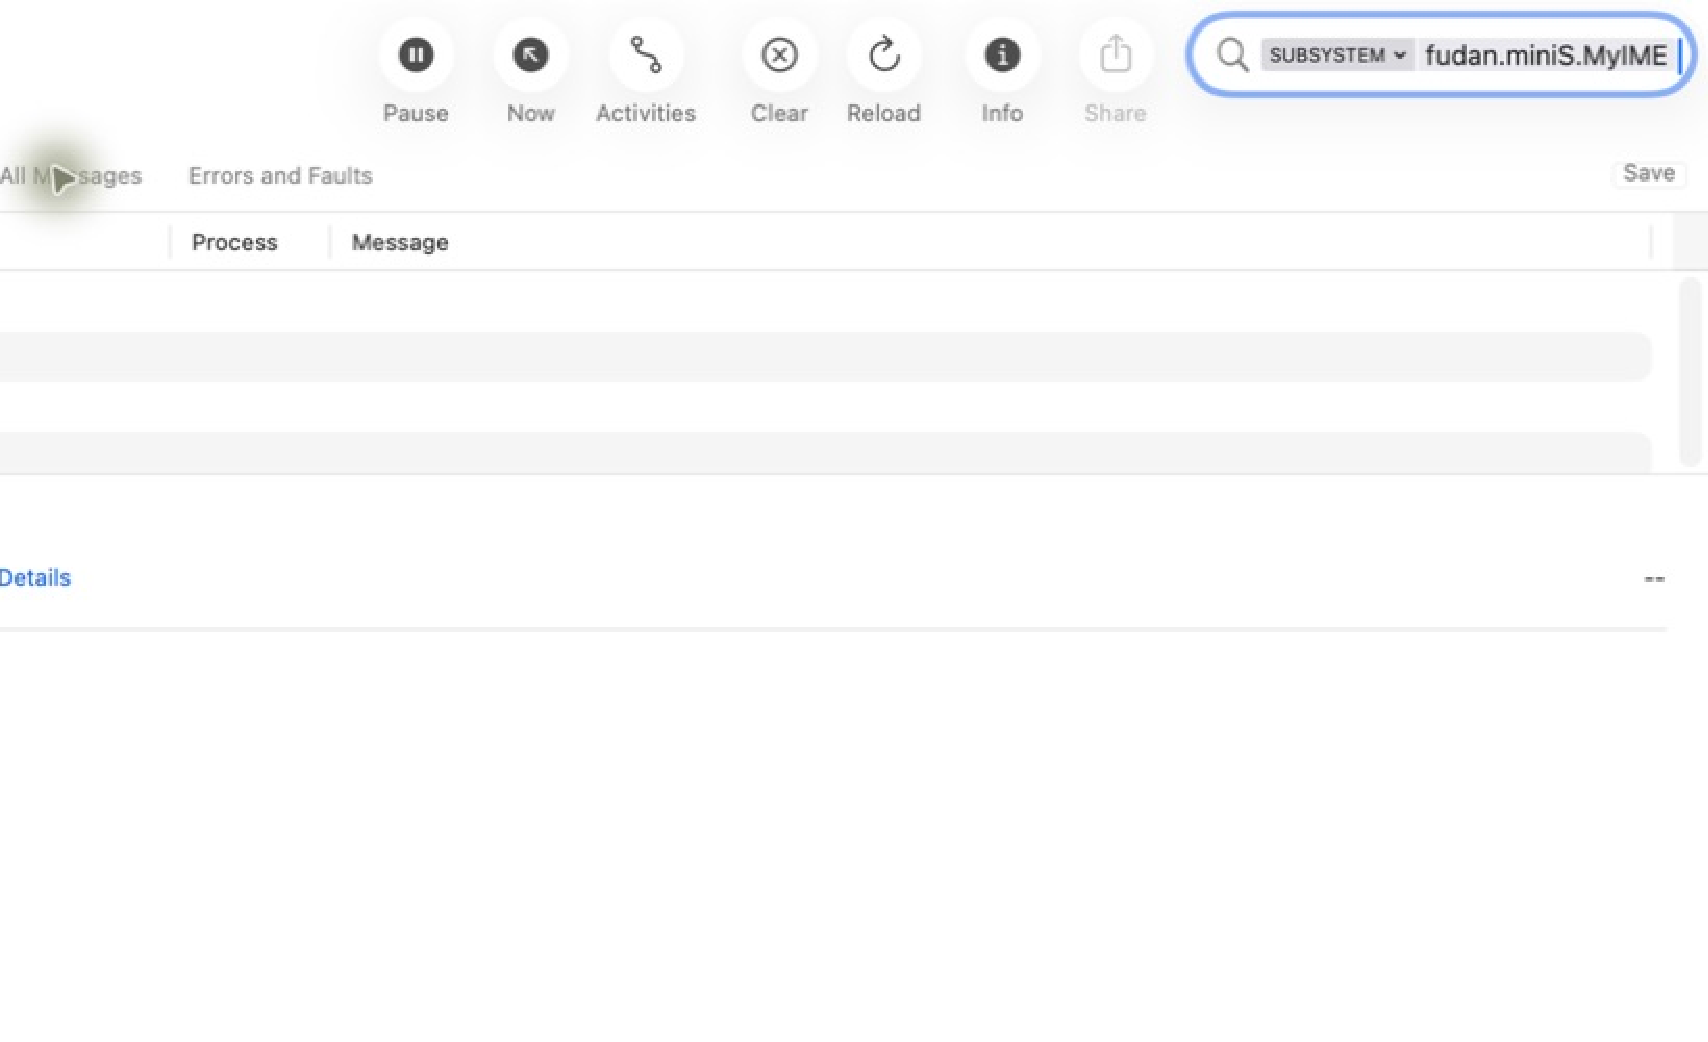
\includegraphics[width=\linewidth]{assets/console-filter.pdf}
  \caption{Console.app 以 subsystem 过滤 MyIME 日志；截图已裁去机器名称}
\end{figure}

一轮复现应形成以下最小证据链：\code{bootstrap server ready} → \code{controller keyDown} → \code{engine candidates=N} → \code{client marked/insert}。若第一项都没有，查进程和 IMKServer；有第一项而没有第二项，查当前输入源与事件入口；有候选却没有客户端调用，查控制器状态和事件返回值。导出日志前必须再次搜索正文样例和用户名，确认脱敏。

\section{诊断问题树}

面对“没有 MyIME”时依次问：

\begin{enumerate}
  \item 安装目录是否存在应用，版本和签名是什么？
  \item TIS 是否枚举到目标输入源 ID？
  \item 当前输入源 ID 是否为 MyIME？
  \item 进程路径是否来自安装目录？IMKServer 是否建立？
  \item 按键进入哪个回调？控制器返回了什么？
  \item 引擎输出候选是否为空？资源库是否完整？
  \item 客户端收到 marked text/insert text 了吗？
\end{enumerate}

面对“候选不对”则从第 5 步开始：归一化 raw、切分路径、SQL 召回、分数分解、后处理和 UI 映射。

\section{隐私友好的日志}

Release 日志可记录：输入长度、路径数量、候选数量、耗时、错误码、应用 Bundle ID 和状态转移；不应默认记录用户完整 raw、候选文本、剪贴板或已提交句子。必要的用户诊断应采用明确同意、短时开启和本地导出。

\begin{concept}[关联 ID]
为一次输入会话生成短关联 ID，使 bootstrap、controller、engine 和 store 日志能够串联，而无需写出正文。例如：\code{session=7F2A, rawLength=8, paths=3, candidates=25, p95Bucket=20ms}。
\end{concept}

\section{死锁与卡顿调试 SOP}

\textbf{先分症状。}崩溃、数据竞争、逻辑死锁和主线程长任务是四类问题，不能只靠同一个工具。复现前固定输入、客户端、系统版本和构建号，并保存正常基线。

\begin{enumerate}
  \item 在 Xcode 的 Scheme→Run→Diagnostics 打开 Thread Sanitizer（TSan），用 Debug 构建重放并发选择、异步学习和数据库故障。TSan 擅长发现未同步的共享内存访问，但不能证明所有逻辑死锁都不存在。命令行可用 \code{xcodebuild ... -enableThreadSanitizer YES test}。TSan 会显著拖慢程序，只用于诊断构建。\footnote{Apple：\url{https://developer.apple.com/documentation/xcode/diagnosing-memory-thread-and-crash-issues-early}}
  \item 若界面已经卡住，在 Xcode 点击 Pause，展开所有线程。记录主线程调用栈、持锁线程和等待栈；若线程 A 等待由 A 自己持有的非递归 \code{NSLock}，就是重入；若 A 等 B、B 又等 A，则画出等待环。不要在锁内调用客户端、SQLite、日志插值闭包或未知回调。
  \item 打开 Main Thread Checker，捕获从后台线程触碰 \code{NSPanel}/SwiftUI 的路径。它检查 UI 线程契约，和 TSan 的数据竞争检查互补。
  \item 对“能动但很慢”选择 Product→Profile→Time Profiler。只录制 10--20 秒：先空闲 3 秒，再输入固定长句，最后空闲 3 秒。按进程过滤 MyIME，展开 Main Thread；重点查 \code{sqlite3_step}、锁等待、候选排序和 SwiftUI 布局是否占据热栈。Apple 也建议用 Time Profiler 分析无响应与挂起。\footnote{Apple：\url{https://developer.apple.com/documentation/xcode/improving-your-app-s-performance/}}
  \item 修改后用相同机器、输入和采样窗口复测，比较 P50/P95 与主线程最重栈，而不是只报告“感觉顺了”。再关闭 Sanitizer 运行一次 Release 配置，排除诊断开销造成的假象。
\end{enumerate}

\begin{warningbox}[NSLock 重入的典型陷阱]
线程在持有 \code{NSLock} 时调用一个看似只读的辅助函数，而该函数为了读取同一状态再次加锁，会永久等待。把锁保护的不变量写在字段旁；锁内只复制/更新小状态，解锁后再调用数据库、客户端和 UI。
\end{warningbox}

\section{诊断工具}

仓库提供输入源检查、注册和本地安装工具。工具输出应被视作辅助证据，而不是绕过正常系统路径的永久依赖。正式版不能靠一个登录守护进程不断强制恢复，因为这会隐藏生命周期设计缺陷。

\lstinputlisting[language=Swift,firstline=1,lastline=120,caption={输入源检查工具示例}]{../../tools/inspect_input_source.swift}

\begin{lab}[故障注入]
分别制造词库缺失、用户库只读、错误输入源 ID 和候选坐标失败。为每个故障写出预期日志和用户可见降级，验证不会让所有按键失效。
\end{lab}

\exercises
\begin{enumerate}
  \item 日志中记录 raw 的 SHA-256 是否绝对安全？为什么？
  \item 设计一个一键生成的本地诊断报告目录结构。
  \item “进程存在但没有回调日志”下一步应收集什么证据？
\end{enumerate}

\begin{summarybox}
好的诊断系统把模糊故障变成逐层证据链，并把可观察性与隐私同时纳入设计，而不是发生问题后临时加 print。
\end{summarybox}


\chapter{隐私、安全与词库许可证}

\begin{goals}
理解输入法的高敏感权限；能够建立完全离线的威胁模型；识别安全输入、日志、更新包、用户数据库和第三方词库中的风险。
\end{goals}

输入法位于所有文本之前，理论上可能接触私人通信、搜索、地址和代码。即使产品承诺离线，也必须用架构和可验证事实支持承诺：没有网络依赖、没有隐蔽上传路径、日志不保存正文、更新包经过签名、用户库权限正确。

\section{威胁模型}

至少考虑以下资产与攻击面：

\begin{itemize}
  \item 用户原始按键、候选选择和提交文本；
  \item 用户词库与上下文数据库；
  \item 应用内置系统词库和替换词库入口；
  \item 安装器的文件替换权限；
  \item 发布服务器、GitHub Release 和 DMG 供应链；
  \item 调试日志、崩溃报告与课堂演示录像。
\end{itemize}

完全离线可以显著缩小攻击面，但不能自动解决本地恶意软件、宽松文件权限、未签名更新和敏感日志。用户数据库应存放在当前用户目录，避免其他普通账户读取；导出时应明确提示内容敏感。

\section{安全输入}

密码字段可能启用 Secure Event Input 或拒绝第三方组合。输入法应尊重该边界，不尝试绕过；无法输入时回退系统安全键盘是正确行为。教学演示禁止在真实密码框记录事件日志。

\section{开源与词库许可}

输入法代码开源不等于所有聚合词库都可以任意再分发。MyIME 的流水线记录来源锁、许可证和派生步骤，应用内附第三方声明。

\lstinputlisting[language=bash,firstline=1,lastline=95,caption={词库来源与许可清单的一部分}]{../../tools/LICENSES.md}

课堂项目应为每个来源记录：名称、URL、版本/提交、许可证、是否修改、输出中保留什么以及再分发义务。无法确认许可的词表不得进入正式发布包。

\begin{lab}[离线审计]
在干净用户账户中运行输入法，使用系统网络观察工具检查进程连接；搜索源码中的 URLSession、Network 和 socket 调用；检查 Release 包中第三方声明与词库来源是否一致。
\end{lab}

\exercises
\begin{enumerate}
  \item “不上传击键”与“完全没有网络请求”有什么区别？
  \item 用户主动导出词库是否改变应用的隐私责任？
  \item 为可下载的离线词库更新包设计签名验证流程。
\end{enumerate}

\begin{summarybox}
输入法的隐私承诺必须由网络边界、日志策略、文件权限、供应链和许可证记录共同支撑。离线是强优势，但不是安全证明的终点。
\end{summarybox}


\chapter{测试体系：从内存词库到跨机器验收}

\begin{goals}
建立单元、集成、性能和人工验收四层测试；掌握 golden、性质测试、故障注入和确定性；把历史故障转化为回归用例。
\end{goals}

输入法核心适合大量自动化测试，系统集成则需要少量高价值人工测试。测试金字塔底层包含切分、排序、用户学习和数据库；中层构建应用并检查资源、签名和架构；顶层在真实客户端敲固定序列。

\figmp{11}{自动化与人工测试的合理比例}

\section{行为测试}

MyIME 的内存词库让测试只包含与行为有关的词。Golden 测试锁定 \code{nihao}→“你好”等核心首选；上下文测试故意让“田七”静态权重更高，再由“今天”上下文把“天气”提升回来。

\lstinputlisting[language=Swift,firstline=103,lastline=174,caption={整句、上下文与续写测试}]{../../MyIME/IMEKit/Tests/IMEKitTests/IMEKitTests.swift}

\section{性质与故障测试}

固定样例覆盖已知场景，性质测试覆盖不变量。例如对随机 ASCII 字符串：引擎不崩溃、耗时不超过预算、消费长度不越界、同输入与同状态结果确定。对损坏数据库：引擎降级，不阻塞基本输入。

\section{性能测试}

性能断言应在可控环境执行，避免把 CI 机器偶发负载当作算法回归。更稳健的做法是记录分布并设置宽松硬门槛，同时在版本间比较相对变化。冷启动、热查询和长句需要分别统计。

\section{跨机器门禁}

发布前必须在不含开发证书、不含旧输入法副本的第二台 Mac 上，从 GitHub Release 下载 DMG，完成安装、注册和 Notes 输入。开发机成功不能替代跨机器验收，因为钥匙串、LaunchServices 缓存和旧构建都可能掩盖问题。

\begin{lab}[把 bug 变成测试]
选择一次历史故障，例如进程被结束后不能恢复、换机后输入源不出现或 Notes 无法组合。先写最小复现，再决定哪一部分能自动化，哪一部分保留为发布清单。
\end{lab}

\exercises
\begin{enumerate}
  \item Golden 测试过多会带来什么维护问题？
  \item 如何测试候选排序确定性？
  \item 为什么跨机器验收属于发布门禁，而不是“有空再测”？
\end{enumerate}

\begin{summarybox}
测试体系要让算法快速回归、系统问题可复现、发布风险可阻断。每个真实故障都应留下自动化测试或明确人工门禁。
\end{summarybox}


\chapter{签名、公证、Universal 2 与 DMG 发布}

\begin{goals}
理解开发签名、Developer ID、公证和装订的区别；能够解释 Universal 2；掌握可重复发布流水线与校验和。
\end{goals}

能在开发机运行的应用不等于可以跨机器分发。公开 DMG 应使用 Developer ID Application 证书签名，提交 Apple 公证，成功后把票据装订到应用或镜像，并验证 Gatekeeper 接受。

\figmp{12}{从测试到公开 DMG 的发布门禁}

\section{签名身份}

Apple Development 证书用于开发调试；Developer ID Application 用于 App Store 外分发。Ad-hoc 签名只证明代码页一致，不建立公开开发者信任。发布脚本必须主动拒绝把 development 或 ad-hoc 构建标为正式版。

\section{Universal 2}

Universal 2 应用同时包含 arm64 和 x86\_64 代码。仅把文件名写成 universal 不够，需要用 \code{lipo -info} 或 \code{file} 检查主可执行文件和嵌入的本地库。SQLite 等系统动态库通常由系统提供，但自带二进制依赖也必须双架构。

\section{发布脚本}

MyIME 的脚本按顺序运行引擎测试、词库验证、构建、架构检查、签名、DMG、公证、装订和 SHA-256。顺序本身就是安全性质：任何前置门禁失败都不应继续发布。

\lstinputlisting[language=bash,firstline=1,lastline=220,caption={正式发布脚本的环境检查与主要门禁}]{../../tools/build-release.sh}

\section{凭据管理}

公证凭据应存入钥匙串 profile，而不是写进脚本或提交到仓库。应用专用密码一旦出现在截图或聊天记录中，应立即撤销并重新生成。课堂作业不要求学生共享教师证书；每组可生成 ad-hoc 演示包，正式公开发布由项目维护者在受控机器执行。

\begin{warningbox}[公证成功不代表功能成功]
公证只证明 Apple 的安全检查接受该二进制，不证明输入源能注册、候选准确或 Notes 可输入。最终门禁仍包含目标机功能验收。
\end{warningbox}

\begin{lab}[验收一个 Release]
对 DMG 依次运行 \code{shasum -a 256}、\code{spctl --assess}、\code{codesign --verify --deep --strict}、\code{xcrun stapler validate}。挂载后检查应用版本、架构与签名团队，再在干净 Mac 安装。
\end{lab}

\exercises
\begin{enumerate}
  \item 签名、公证和装订分别解决什么问题？
  \item 为什么发布凭据不能通过环境变量明文保存在 CI 日志？
  \item 设计一份可由第三方复核的 Release 清单。
\end{enumerate}

\begin{summarybox}
正式发布是一条不可跳步的证据链。测试、双架构、Developer ID、Apple 公证、票据装订、校验和和跨机器输入共同定义“可下载版本”。
\end{summarybox}


\chapter{维护真实输入法：技术债与演进边界}

\begin{goals}
能够评审控制器和安装器中的复杂度；区分教学最小实现与生产兼容代码；设计版本迁移、文档同步和未来功能边界。
\end{goals}

MyIME 作为教学案例的价值在于它既有清晰核心，也暴露真实复杂度。\sourcefile{Engine.swift}、\sourcefile{MyIMEInputController.swift} 和 \sourcefile{SelfInstaller.swift} 已经包含大量策略。继续增加双拼、云更新或移动平台前，应先检查模块边界，而不是把新分支堆进控制器。

\section{复杂度地图}

\begin{center}
\begin{tabularx}{\linewidth}{p{3cm}X X}
\toprule
模块 & 当前职责 & 演进建议 \\
\midrule
InputController & 事件、组合、候选导航、客户端适配、英文辅助 & 抽出 InputAction 与 CompositionState，降低分支耦合 \\
Engine & 切分协调、词查询、评分、词格、上下文、学习 & 保持纯逻辑；为评分解释和策略注入留接口 \\
SQLiteStore & 系统查询、统计模型、用户库 & 分离只读 schema 与用户迁移版本 \\
SelfInstaller & 复制、注册、旧版迁移、重启 & 用明确安装阶段和错误类型替代隐式布尔状态 \\
候选窗口 & SwiftUI 渲染与 AppKit 窗口定位 & 增加可访问性与多屏快照测试 \\
\bottomrule
\end{tabularx}
\end{center}

\section{规格、实现与测试同步}

仓库中的 \sourcefile{SPEC.md} 描述目标，\sourcefile{FOOLPROOFING.md} 描述门禁，README 描述用户能力，代码是实际行为。它们可能随版本产生漂移。维护者应给每项功能标记 implemented、planned 或 removed，并把用户可见变化写入版本说明。

\section{功能边界}

双拼会改变切分与设置，但不必改变 IMK 生命周期；云词库会改变隐私承诺和更新安全；语音输入引入音频权限与服务端/本地模型；移动端输入法则是不同平台架构。评审新功能时先问它改变哪一层契约，再决定是否仍属于同一个产品。

\begin{concept}[教学版与完整版共存]
最好的教材仓库不是把生产代码削成玩具，而是保留两个视图：章节化的教学版展示关键原理，完整版展示边界条件和发布现实。学生先能解释，再能维护。
\end{concept}

\section{把无障碍作为回归契约}

候选列表的“能看见、能点击”不等于可访问。每个候选行应是独立无障碍元素，标签读出序号与候选词，当前高亮项增加 \code{.isSelected} trait；辅助说明放在 hint，不要把词频、调试分数等噪声塞进主标签。SwiftUI 示例见第 7 章。

当方向键改变高亮时，可按需发送 \code{NSAccessibility.announcementRequestedNotification}，\code{userInfo} 中提供 announcement 与 priority。\footnote{Apple：\url{https://developer.apple.com/documentation/appkit/nsaccessibilityannouncementrequestednotification}}公告必须节流：按键长按时只读最终稳定项，避免 VoiceOver 被消息队列淹没。非激活 \code{NSPanel} 不应抢走宿主编辑器焦点；关闭候选窗后，VoiceOver 焦点仍应留在原文本控件。

每次改候选 UI 至少回归：VoiceOver 开/关、键盘全访问、提高对比度、减少透明度、浅色/深色、多屏与放大显示。自动化测试可验证 label、selected trait 和稳定候选索引，人工测试负责朗读顺序、焦点保持与语速下的可理解性。

\begin{lab}[架构评审]
选择一个计划功能（双拼、词库导入、诊断面板或用户词导出），写一页变更契约：目标、涉及模块、不改变的行为、数据迁移、测试和发布风险。禁止先写代码。
\end{lab}

\exercises
\begin{enumerate}
  \item 哪些控制器状态可以抽成纯 Swift 状态机？
  \item 加入双拼时，Candidate 的 pinyinPath 是否仍足够？
  \item 如何避免教材行号随源码变化失效？提出一种自动检查办法。
\end{enumerate}

\begin{summarybox}
真实输入法的维护重点不是持续增加功能，而是守住系统、算法、存储和发布契约。教学最小版解释原理，完整版本训练工程判断。
\end{summarybox}
